\documentclass[a4paper,12pt]{article}

\usepackage{cmap}					% поиск в PDF
\usepackage[utf8]{inputenc}
\usepackage[T2A]{fontenc}
\usepackage[english,russian]{babel}
\usepackage[autostyle]{csquotes}
\usepackage{graphicx}
\usepackage{caption}
\usepackage{indentfirst}
\usepackage{listings}
\usepackage{float}
\usepackage[authoryear,round]{natbib}
\usepackage{biblatex}
\usepackage{amsmath,amsfonts,amssymb,amsthm,mathtools} 
\graphicspath{ {images/} }
\author{Казакова Элиза}
\date{\today}
\usepackage[left=2cm,right=2cm,top=2cm,bottom=2cm,bindingoffset=0cm]{geometry}
\newcommand{\anonsection}[1]{\section*{#1}\addcontentsline{toc}{section}{#1}}
\begin{document} % Конец преамбулы, начало текста.
	
	\begin{titlepage}
		\fontsize{12pt}{12pt}\selectfont
		\noindent \begin{minipage}{0.15\textwidth}
			
\includegraphics[width=\linewidth]{ MGTU.png}
		\end{minipage}
		\noindent\begin{minipage}{0.9\textwidth}\centering
			\textbf{Министерство науки и высшего образования Российской Федерации}\\
			\textbf{Федеральное государственное бюджетное образовательное учреждение высшего образования}\\
			\textbf{«Московский государственный технический университет имени Н.Э.~Баумана}\\
			\textbf{(национальный исследовательский университет)»}\\
			\textbf{(МГТУ им. Н.Э.~Баумана)}
		\end{minipage}
		
		\noindent\rule{18cm}{3pt}
		\newline\newline
		\noindent 
		ФАКУЛЬТЕТ 
		\underline{«Информатика и системы управления»} \newline\newline
		
		\noindent КАФЕДРА \underline{«Программное обеспечение ЭВМ и информационные технологии»}\newline\newline\newline\newline\newline\newline\newline
		
		\begin{center}
			\Large\textbf{\qquad\qquad Отчет по лабораторной работе №3} \newline
		\end{center}
		
		\begin{center}
			\textbf{\qquad\qquad       По дисциплине: Анализ Алгоритмов} \newline
		\end{center}
		\textbf{\qquad\qquad\qquad Тема: } \underline{Трудоемкость алгоритмов сортировки} \newline\newline\newline
		\textbf{\qquad Студент} \underline{Казакова Э.М.~~~~~~~~~~~~~~~~~~~~~~~~~~~~~~~~~}\newline\newline
		\textbf{\qquad Группа} \underline{ИУ7-56Б~~~~~~~~~~~~~~~~~~~~~~~~~~~~~~~~~~~~~~~~~~~~~~~~~~~~~}\newline\newline
		\textbf{\qquad Оценка (баллы)} \underline{~~~~~~~~~~~~~~~~~~~~~~~~~~~~~~~~~~~~~~~~~~~~~~~~~~~}\newline\newline
		\textbf{\qquad Преподаватели} \underline{Волкова Л.Л., Строганов Ю.В.~~~~~~~~~~}\newline
		
		\begin{center}
			\vfill
			Москва~---~\the\year
			~г.
		\end{center}
	\end{titlepage}
	
	\tableofcontents
	\newpage
	
	\anonsection{Введение}
	\hfill
	
	В настоящее время необходимо сортировать большие объемы данных.
	Для этой цели существуют алгоритмы сортировки, которые упорядочивают
	элементы в списке.
	[1] Сортировкой называют процесс перегруппировки заданной последовательности (кортежа) объектов в некотором определенном порядке. Определенный порядок (например, упорядочение в алфавитном порядке, по возрастанию или убыванию количественных характеристик, по классам, типам
	и.т.п.) в последовательности объектов необходимо для удобства работы с
	этим объектом.
	
	Целью данной лабораторной работы является изучение и реализация алгоритмов сортировки, исследование их трудоемкости.
	
	Задачи данной лабораторной работы:
	\begin{enumerate}
		\item изучить алгоритмы сортировки пузырьком, вставками, выбором;
		\item реализовать алгоритмы сортировки пузырьком, вставками, выбором;
		\item дать оценку трудоёмкости (для двух алгоритмов сделать вывод трудоёмкости);
		\item провести замеры процессорного времени работы для лучшего, худшего и произвольного случая.
	\end{enumerate}

	\newpage
	\section{Аналитическая часть}
	
	\hfill
	
	В данной части будут рассмотрены основные теоретические аспекты, связанные с алгоритмами сортировок пузырьком, вставками, выбором.
	
	\subsection{Сортировка вставками}
	\hfill
	
	Сортировка вставками[2] — это простой алгоритм сортировки. Суть его заключается в том что, на каждом шаге алгоритма мы берем один из элементов массива, находим позицию для вставки и вставляем. Стоит отметить что массив из 1-го элемента считается отсортированным.
	
	Сортировка вставками наиболее эффективна когда массив уже частично отсортирован и когда элементов массива не много. Данный алгоритм можно ускорить при помощи использования бинарного поиска для нахождения места текущему элементу в отсортированной части.
	
	\subsection{Сортировка выбором}
	\hfill

	Один из самых простых методов сортировки работает следующим образом: находим наименьший элемент в массиве и обмениваем его с элементом находящимся на первом месте. Потом повторяем процесс со второй позиции в файле и найденный элемент обмениваем со вторым элементном и так далее пока весь массив не будет отсортирован. Этот метод называется сортировка выбором, поскольку он работает, циклически выбирая наименьший из оставшихся элементов. Главное отличие сортировки выбором от сортировки вставками: в сортировке вставками мы извлекаем из неотсортированной части массива любой элемент и вставляем его на своё место в отсортированной части. В сортировке выбором мы целенаправленно ищем максимальный элемент(или минимальный), которым дополняем отсортированную часть массива. Во вставках мы ищем куда вставить очередной элемент, а в выборе — мы заранее уже знаем в какое место поставим, но при этом требуется найти элемент, этому месту соответствующий.
	
	\subsection{Сортировка пузырьком}
	\hfill
	
	Алгоритм проходит по массиву n-1 раз до тех пор, пока массив не будет
	полностью отсортирован. В каждом проходе элементы попарно сраниваются и,
	при необходимости, меняются местами. При каждом проходе алгоритма по
	внутреннему циклу, очередной наибольший элемент ставится на своё место в
	конец неотсортированного массива. Таким образом наибольшие элементы
	"всплывают"как пузырёк.
		
	\subsection{Вычисление сложности алгоритма}
	\hfill
	
	В рамках данной работы используется следующая модель вычислений:\\
	\begin{enumerate}
		\item базовые операции имеют трудоемкость 1 (<, >, =, <=, =>, ==, +, -, *, /, \%, \&, +=, -=, *=, /=,  [ ]);\\
		\item операторы if, else if имеют трудоемкость $F_{if} = F_{body} + F_{cheсk}$,  $F_{body}$ - трудоемкость операций тела оператора,  $F_{cheсk}$ - трудоемкость проверки условия;\\
		\item оператор else имеет трудоемкость $F_{body}$;\\
		\item оператор for имеет трудоемкость  $F_{for} = 2 + N \cdot (F_{body} + F_{cheсk})$, где $F_{body}$ – трудоемкость операций в теле цикла.\\
	\end{enumerate}

	\newpage
	\section{Конструкторская часть}
	\hfill
	
	В данном разделе будут рассмотрены схемы алгоритмов сортировок пузырьком, вставками и выбором. 
	
	\subsection{Схемы алгоритмов}
	\hfill
	
	На рисунке 1 представлена схема алгоритма сортировки пузырьком.
	\begin{figure}[H]
		\centering
		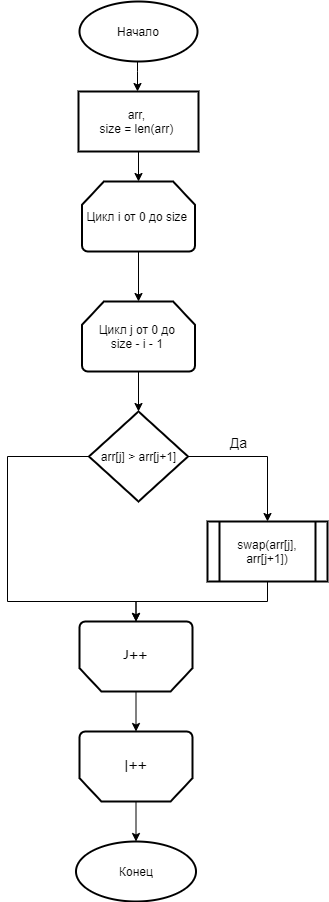
\includegraphics[scale=1.6]{bubble.png}
		\captionsetup{justification=centering}
		\caption{Схема алгоритма сортировки пузырьком}
		\label{Рис 1}
	\end{figure}

	На рисунке 2 представлена схема алгоритма сортировки вставками.
	\begin{figure}[H]
		\centering
		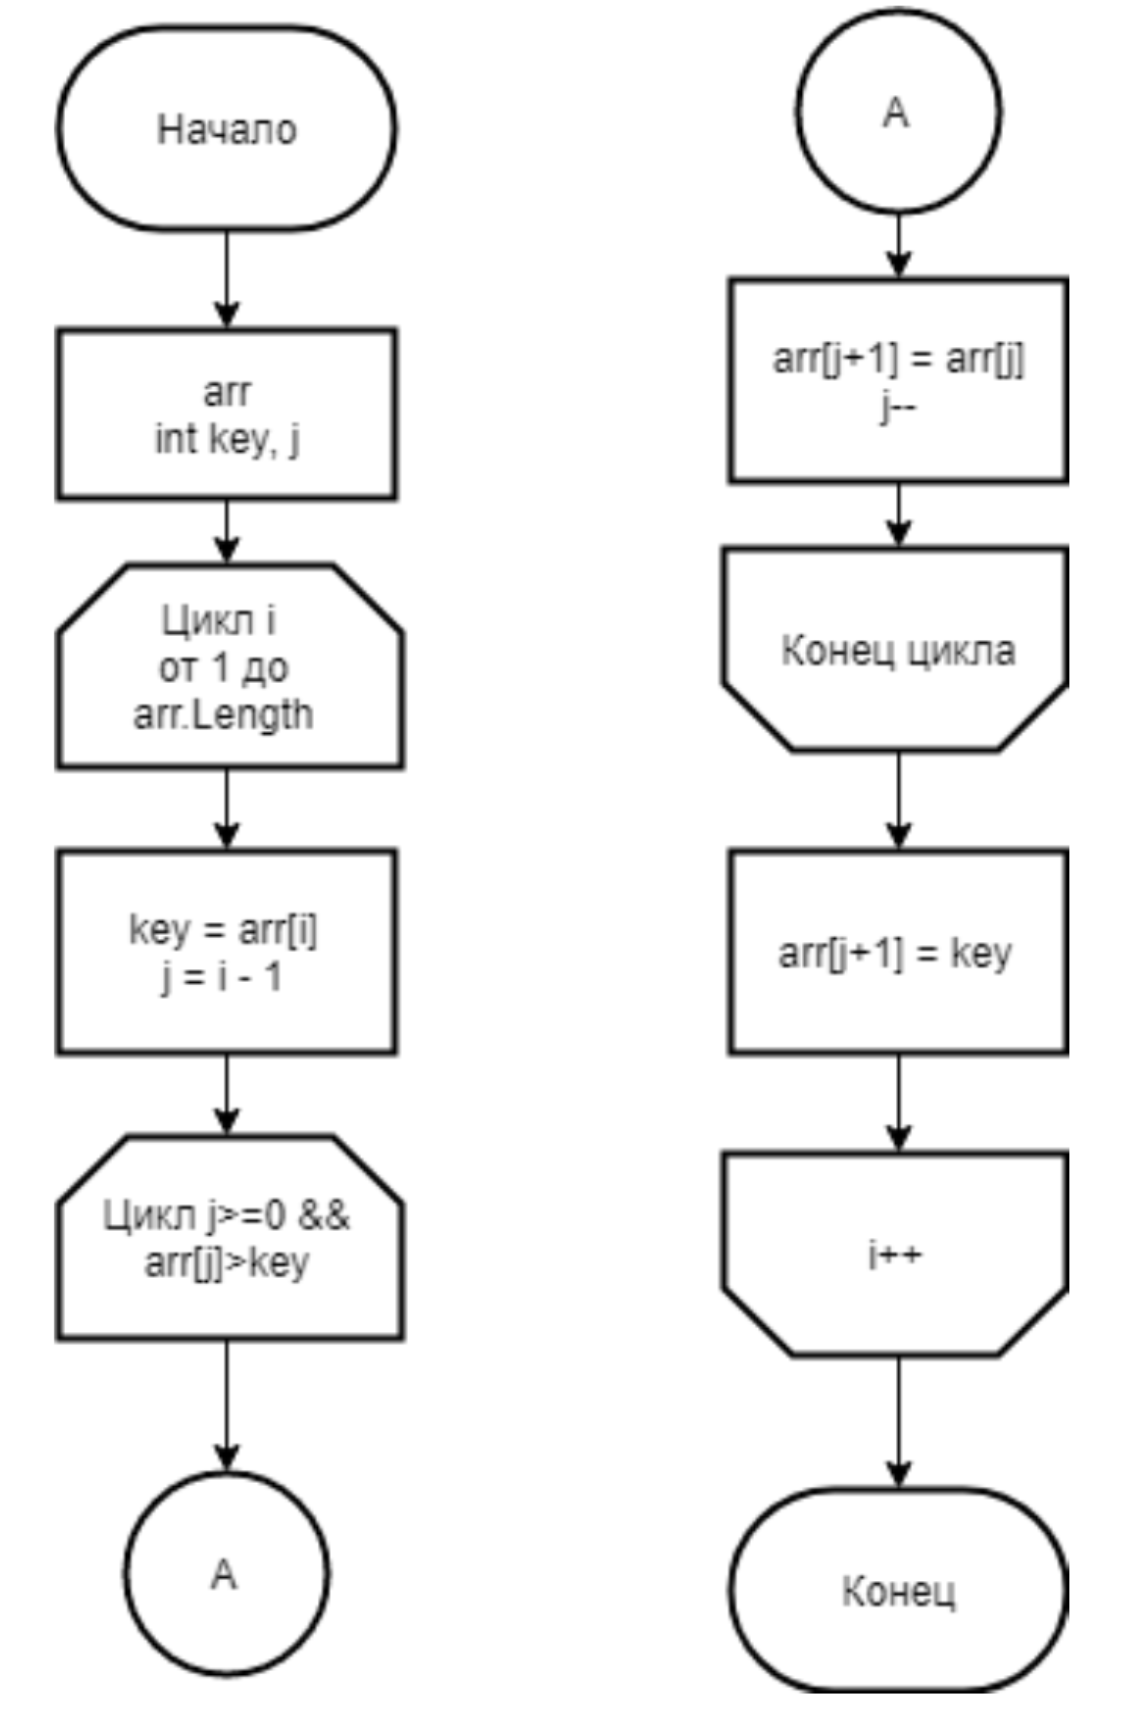
\includegraphics{insert.png}
		\captionsetup{justification=centering}
		\caption{Схема алгоритма сортировки вставками}
		\label{Рис 2}
	\end{figure}
	На рисунке 3 представлена схема алгоритма сортировки выбором.
	\begin{figure}[H]
		\centering
		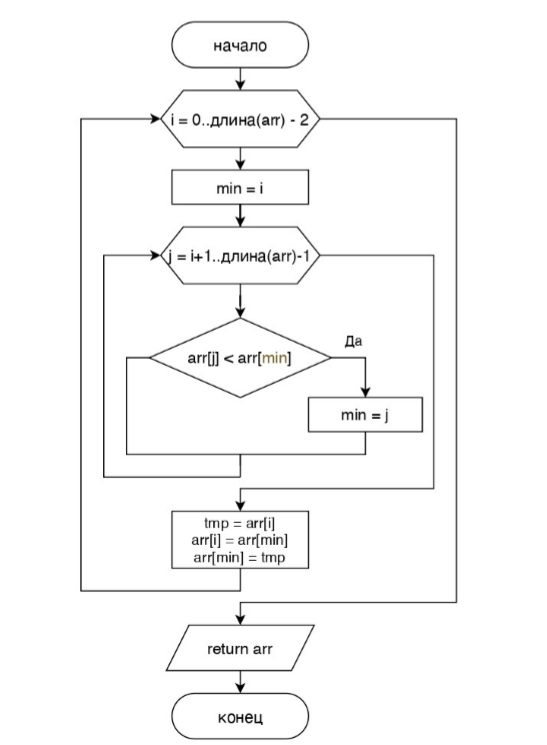
\includegraphics{min.png}
		\captionsetup{justification=centering}
		\caption{Схема алгоритма сортировки выбором}
		\label{Рис 3}
	\end{figure}
	\newpage
	\section{Технологическая часть}
	\hfill
	
	В данном разделе будут рассмотрены требования к программному обеспечению, средства реализации и представлен листинг кода.
	\subsection{Требования к программному обеспечению}
	\hfill
	
	ПО должно предоставлять возможность ввода массива, на выходе пользователь должен получить результат сортировки массива, произведенной тремя алгоритмами. Также ПО должно обеспечить вывод замеров времени работы каждого из алгоритмов в худшем, лучшем и произвольном случаях
	
	\subsection{Средства реализации}
	\hfill
	
	В данной работе используется язык программирования Python, так как ЯП позволяет написать программу за кратчайшее время.В качестве среды разработки выбрана IDLE. Для замеров времени была выбран метод process\_time() модуля time[3], он возвращает значение (в долях секунды) системного процессорного времени текущего процесса.
	
	\subsection{Листинг кода}
	\hfill
	В листингах 3.1 - 3.3 представлена реализация алгоритма сортировки пузырьком,  вставками и выбором.
	\lstset{ %
		language=Python,                % Язык программирования 
		numbers=left,                   % С какой стороны нумеровать                           
	}
	\textbf{\\Листинг 3.1 -- Алгоритм сортировки пузырьком}
	
	\begin{lstlisting}
	def bubble_sort(arr):
		start_time = time.process_time()
		for i in range(len(arr)):
			for j in range(0, len(arr)-i-1):
				if arr[j] > arr[j+1]:
					arr[j], arr[j+1] = arr[j+1], arr[j]
		t = time.process_time() - start_time
		return t	
	\end{lstlisting}
	\textbf{\\Листинг 3.2 -- Алгоритм сортировки вставками }
	
	\begin{lstlisting}
	def insertion_sort(arr):
		start_time = time.process_time()
		for i in range(1, len(arr)):
			j = i - 1
			key = arr[i]	
			while j >= 0 and arr[j] > key:
				arr[j + 1] = arr[j]
				j -= 1
			arr[j + 1] = key
		t = time.process_time() - start_time
		return t
	\end{lstlisting}
	
	\textbf{\\Листинг 3.3 -- Алгоритм сортировки выбором}
	
	\begin{lstlisting}
	def selection_sort(arr):
		start_time = time.process_time()
		for i in range(0, len(arr) - 1):
			min = i
			for j in range(i + 1, len(arr)):
				if arr[j] < arr[min]:
					min = j
			arr[i], arr[min] = arr[min], arr[i]
		t = time.process_time() - start_time
		return t
	\end{lstlisting}
	
	\subsection{Тестирование}
	\hfill
	
	В данном разделе будут показаны результаты тестирования
	Всего было реализовано 5 тестовых случаев:
	\begin{enumerate}
		\item размер массива равен 0;
		\item сравнение работы все трех алгоритмов на уже отсортированных
		значениях массива;
		\item сравнение работы все трех алгоритмов на обратно отсортированных
		значениях массива;
		\item сравнение работы все трех алгоритмов на случайных значениях массива;
	\end{enumerate}
	
	На рисунках 4-7 представлены результаты работы программы при вводе различных входных тестовых данных.
	
	\begin{figure}[H]
		\centering
		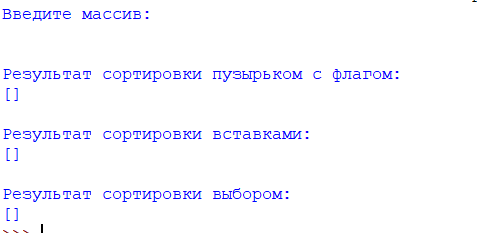
\includegraphics{res1.png}
		\captionsetup{justification=centering}
		\caption{Результат программы при нулевом размере массива}
		\label{Рис 4}
	\end{figure}

	\begin{figure}[H]
		\centering
		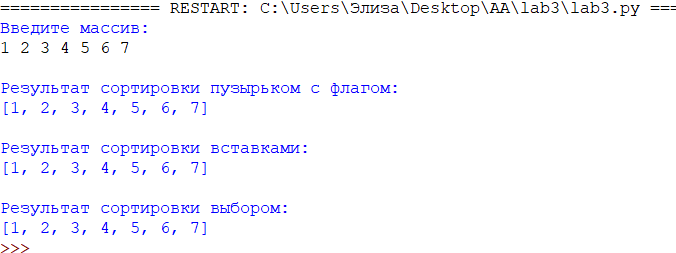
\includegraphics{res2.png}
		\captionsetup{justification=centering}
		\caption{Результат программы при уже отсортированных значениях массива}
		\label{Рис 5}
	\end{figure}
	
	\begin{figure}[H]
		\centering
		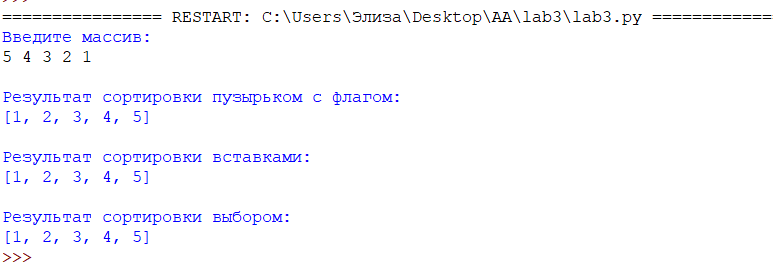
\includegraphics{res3.png}
		\captionsetup{justification=centering}
		\caption{Результат программы при обратно отсортированных значениях массива}
		\label{Рис 6}
	\end{figure}

	\begin{figure}[H]
		\centering
		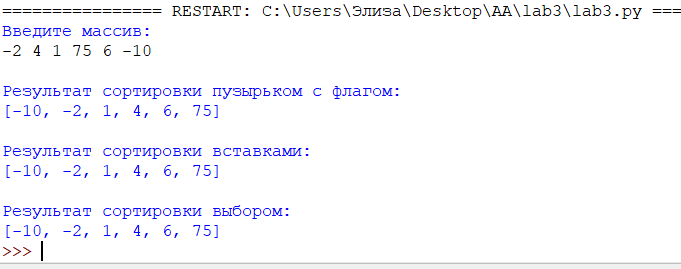
\includegraphics{res4.png}
		\captionsetup{justification=centering}
		\caption{Результат программы при случайных значениях массива}
		\label{Рис 7}
	\end{figure}

    
    
    \newpage

	\section{Экспериментальная часть}
	\hfill
	
	В данной части производится экспериментальное сравнение работы трех реализованных алгоритмов (зависимость времени выполнения от размеров массива и лучшего, произвольного или худшего способа заполнения массива).
	
	\subsection{Сравнение времени работы}	
	\hfill
	
	На графиках (рисунки 8 - 10) представлено сравнение времени работы алгоритмов сортировки на массивах разных размеров. Для лучшего случая массивы заполняются в порядке возрастания числами от -1000 до 1000, для худшего случая - в порядке убывания от -1000 до 1000, для произвольного случая - случайно сгенерированными числами в диапазоне от -1000 до 1000. Для построения графиков генерировались массивы размерами от 0 до 6000.
	
	На рисунках 4-7 представлены результаты работы программы при вводе различных входных тестовых данных.
	
	\begin{figure}[H]
		\centering
		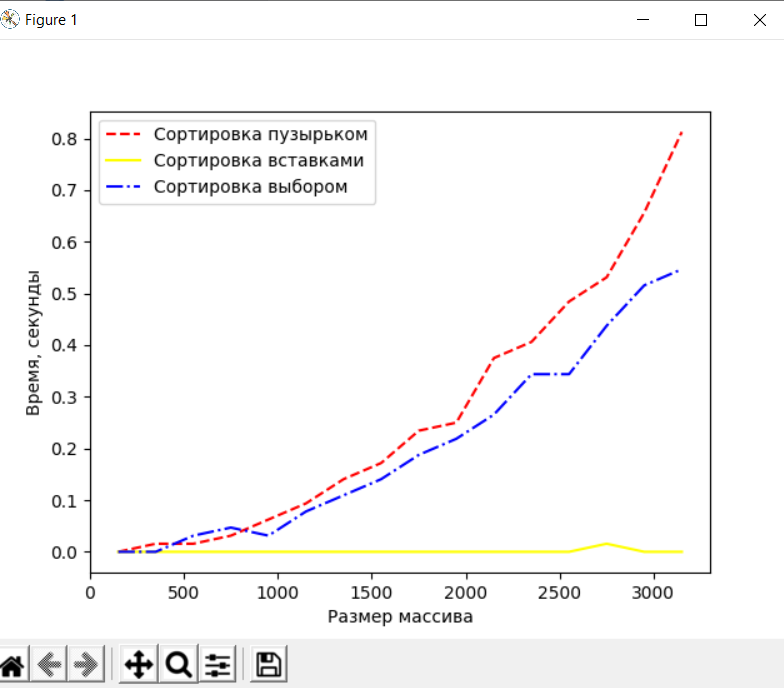
\includegraphics[scale=0.6]{test1.png}
		\captionsetup{justification=centering}
		\caption{Сравнение по времени работы реализации алгоритмов сортировки пузырьком, вставками, выбором (лучший случай)}
		\label{Рис 8}
	\end{figure}
	
	\begin{figure}[H]
		\centering
		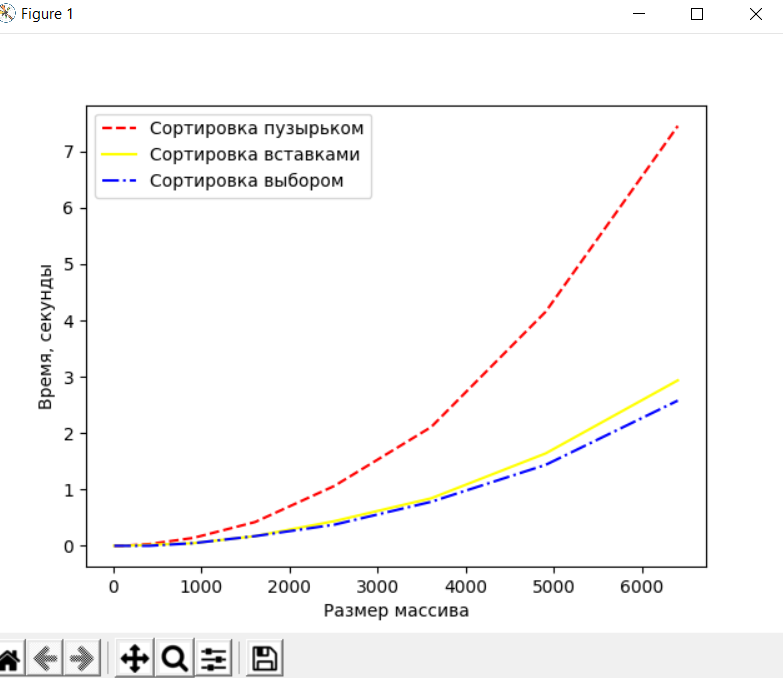
\includegraphics[scale=0.6]{test2.png}
		\captionsetup{justification=centering}
		\caption{Сравнение по времени работы реализации алгоритмов сортировки пузырьком, вставками, выбором (произвольный случай)
		}
		\label{Рис 9}
	\end{figure}
	
	\begin{figure}[H]
		\centering
		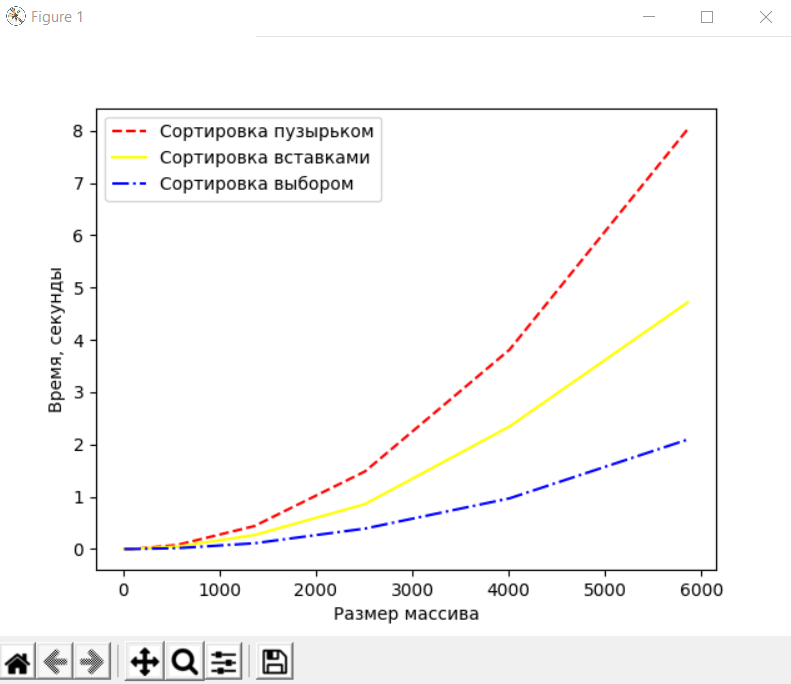
\includegraphics[scale=0.6]{test3.png}
		\captionsetup{justification=centering}
		\caption{Сравнение по времени работы реализации алгоритмов сортировки пузырьком, вставками, выбором (худший случай)}
		\label{Рис 10}
	\end{figure}
	
	
	\subsection{Оценка трудоемкости алгоритмов сортировок}
	\hfill
	
	Далее будет приведены оценки трудоемкости алгоритмов сортировки.

	\begin{enumerate}
		\item Алгоритм сортировки пузырьком. \\
		\hspace*{5mm} {\bf Лучший случай: } Массив отсортирован; не произошло ни одного обмена за 1 проход -> выходим из цикла.
		\\ Трудоемкость: 1 + 1 + 2 + {\it n} * (2 + 7 + 1 + 3) = 13n + 4 = {\it O(n)}.
		\\ \hspace*{5mm} {\bf Худший случай: } Массив отсортирован в обратном порядке; в каждом случае происходил обмен.
		\\ Трудоемкость: 1 + 1 + 2 + {\it n} * ({\it n} * (7 + 5 + 1 + 3) + 1 + 1) = 16$n^2$ + 2n + 4 = {\it O($n^2$)}.
		\item Алгоритм сортировки вставками.\\
		\hspace*{5mm} {\bf Лучший случай: } Массив отсортирован. При этом все внутренние циклы состоят всего из одной итерации.
		\\ Трудоемкость: T(n) = 3n + ((2 + 2 + 4 + 2) * (n - 1)) = 3n + 10(n - 1) = 13n - 10 = {\it O(n)}.
		\\ \hspace*{5mm} {\bf Худший случай: } Массив отсортирован в обратном порядке; каждый новый элемент сравнивается со всеми в отсортированной последовательности. Все внутренние циклы будут состоять из j итераций.
		\\ Трудоемкость:  T(n) = 3n + (2 + 2)(n - 1) + 4($\frac{n(n+1)}{2}$) - 1) + 5$\frac{n(n-1)}{2}$ + 3(n-1) = 3n + 4n - 4 + 2$n^2$ + 2n - 4 + 2.5$n^2$ - 2.5n + 3n - 3 = 4.5$n^2$ + 9.5n - 11 = {\it O($n^2$)}.
		
		\item Алгоритм сортировки выбором.\\
		\hspace*{5mm} {\bf Лучший случай: } $O(N^{2})$
		\\ \hspace*{5mm} {\bf Худший случай: } $O(N^{2})$.	
	\end{enumerate}	
	
	\subsection{Выводы}
	\hfill

	В результате проведенного эксперимента был получен следующий вывод: в лучшем, худшем, произвольном случае сортировка пузырьком оказалась самой медленной. Сортировка вставками в лучшем случае работает быстрее всего. В худшем случае сортировка выбором является самой быстрой. В произвольном случае время работы сортировок вставками и выбором сопоставимо.
	
	\newpage
	
	\anonsection{Заключение}
	\hfill
	
	В ходе лабораторной работе были исследованы алгоритмы сортировок: выбором, пузырьком и вставками. При выполнении лабораторной работе цель была достигнута: были изучены и реализованы алгоритмы сортировки, исследована их трудоемкость.\\
	Также были выполнены следующие задачи: 
	
	\begin{enumerate} 
		\item были изучены алгоритмы сортировки пузырьком, вставками, выбором;
		\item были реализованы алгоритмы сортировки пузырьком, вставками,выбором;
		\item была дана оценка трудоёмкости в лучшем, произвольном и худшем случае;
		\item были проведены замеры процессорного времени работы для лучшего, худшего и произвольного случая.
	\end{enumerate}

	
	\newpage
	 \begin{thebibliography}{}
		\bibitem{} Глушко. Алгоритм сортировки [Электронный ресурс]. - Режим доступа: https://works.doklad.ru/view/MeaUSqCgyps.html.(дата обращения: 23.01.2021)
		
		\bibitem{} В мире алгоритмов: Сортировка Вставками [Электронный ресурс]. - Режим доступа: https://habr.com/ru/post/181271/ (дата обращения: 23.01.2021)
		
		\bibitem{} Златопольский Д.М. Основы программирования на языке Python. – М.: ДМК Пресс, 2017. – 284 с.
	\end{thebibliography} 
	
\end{document} % Конец текста.

